%%%%%%%%%%%%%%%%%%%%%%%%%%%%%%%%%%%%%%%%%
% Short Sectioned Assignment
% LaTeX Template
% Version 1.0 (5/5/12)
%
% This template has been downloaded from:
% http://www.LaTeXTemplates.com
%
% Original author:
% Frits Wenneker (http://www.howtotex.com)
%
% License:
% CC BY-NC-SA 3.0 (http://creativecommons.org/licenses/by-nc-sa/3.0/)
%
%%%%%%%%%%%%%%%%%%%%%%%%%%%%%%%%%%%%%%%%%

%----------------------------------------------------------------------------------------
%	PACKAGES AND OTHER DOCUMENT CONFIGURATIONS
%----------------------------------------------------------------------------------------

% !TeX spellcheck = es_ES
\documentclass[paper=a4, fontsize=11pt]{scrreprt} % A4 paper and 11pt font size

\usepackage[spanish]{babel}
\usepackage[utf8]{inputenc}

\usepackage[T1]{fontenc} % Use 8-bit encoding that has 256 glyphs
\usepackage{fourier} % Use the Adobe Utopia font for the document - comment this line to return to the LaTeX default

\usepackage{amsmath,amsfonts,amsthm} % Math packages
\usepackage{sectsty} % Allows customizing section commands

\usepackage[pdftex]{graphicx}

\usepackage{listings}

\usepackage{calc}

\usepackage{appendix}

\newlength{\imgwidth}

\newcommand\scalegraphics[1]{
    \settowidth{\imgwidth}{\includegraphics{#1}}
    \setlength{\imgwidth}{\minof{\imgwidth}{\textwidth}}
    \includegraphics[width=\imgwidth]{#1}
}

\allsectionsfont{\centering \normalfont\scshape} % Make all sections centered, the default font and small caps
\usepackage{float}
\usepackage{fancyhdr} % Custom headers and footers
\pagestyle{fancyplain} % Makes all pages in the document conform to the custom headers and footers
\fancyhead{} % No page header - if you want one, create it in the same way as the footers below
\fancyfoot[L]{} % Empty left footer
\fancyfoot[C]{} % Empty center footer
\fancyfoot[R]{\thepage} % Page numbering for right footer
\renewcommand{\headrulewidth}{0pt} % Remove header underlines
\renewcommand{\footrulewidth}{0pt} % Remove footer underlines
\setlength{\headheight}{13.6pt} % Customize the height of the header

\numberwithin{equation}{section} % Number equations within sections (i.e. 1.1, 1.2, 2.1, 2.2 instead of 1, 2, 3, 4)
\numberwithin{figure}{section} % Number figures within sections (i.e. 1.1, 1.2, 2.1, 2.2 instead of 1, 2, 3, 4)
\numberwithin{table}{section} % Number tables within sections (i.e. 1.1, 1.2, 2.1, 2.2 instead of 1, 2, 3, 4)

\setlength\parindent{0pt} % Removes all indentation from paragraphs - comment this line for an assignment with lots of text

\def\ScaleIfNeeded{
    \ifdim\Gin@nat@width>\linewidth
    \linewidth
    \else
    \Gin@nat@width
    \fi
}


\usepackage[usenames,dvipsnames]{color}
% This is the color used for MATLAB comments below
\definecolor{MyDarkGreen}{rgb}{0.0,0.4,0.0}

% For faster processing, load Matlab syntax for listings
\lstloadlanguages{Matlab}
\lstset{language=Matlab,                        % Use MATLAB
    columns=fullflexible,
    frame=single,                           % Single frame around code
    basicstyle=\tiny\ttfamily,             % Use small true type font
    keywordstyle=[1]\color{Blue}\bf,        % MATLAB functions bold and blue
    keywordstyle=[2]\color{Purple},         % MATLAB function arguments purple
    keywordstyle=[3]\color{Blue}\underbar,  % User functions underlined and blue
    identifierstyle=,                       % Nothing special about identifiers
    % Comments small dark green courier
    commentstyle=\usefont{T1}{pcr}{m}{sl}\color{MyDarkGreen}\small,
    stringstyle=\color{Purple},             % Strings are purple
    showstringspaces=false,                 % Don't put marks in string spaces
    tabsize=5,                              % 5 spaces per tab
    %
    %%% Put standard MATLAB functions not included in the default
    %%% language here
    morekeywords={xlim,ylim,var,alpha,factorial,poissrnd,normpdf,normcdf},
    %
    %%% Put MATLAB function parameters here
    morekeywords=[2]{on, off, interp},
    %
    %%% Put user defined functions here
    morekeywords=[3]{},
    %
    morecomment=[l][\color{Blue}]{...},     % Line continuation (...) like blue comment
    numbers=left,                           % Line numbers on left
    firstnumber=1,                          % Line numbers start with line 1
    numberstyle=\tiny\color{Blue},          % Line numbers are blue
    stepnumber=1                            % Line numbers go in steps of 5
}

%----------------------------------------------------------------------------------------
%	TITLE SECTION
%----------------------------------------------------------------------------------------

\newcommand{\horrule}[1]{\rule{\linewidth}{#1}} % Create horizontal rule command with 1 argument of height

\title{
    \normalfont \normalsize 
    \textsc{Robótica Industrial} \\ [25pt] % Your university, school and/or department name(s)
    \horrule{0.5pt} \\[0.4cm] % Thin top horizontal rule
    \huge Práctica 4: Sistemas Analógicos y de control \\ % The assignment title
    \horrule{2pt} \\[0.5cm] % Thick bottom horizontal rule
}

\author{Juan Antonio Aldea Armenteros} % Your name

\date{\normalsize\today} % Today's date or a custom date

\begin{document}
    
    \maketitle % Print the title
    \chapter{Introducción a Simulink. Sistemas Analógicos}
    En los siguientes apartados se realizará un estudio del comportamiento de los sistemas analógicos de segundo orden ante diversos tipos de excitación utilizando la herramienta Simulink.
    \section{Sistemas de Segundo Orden}
    Se estudiará la respuesta a una entrada tipo escalón unitario del sistema cuya función de trasferencia es la siguiente
    \begin{align}
        G(s) = \frac{\omega_n^2}{s^2+2\delta\omega_ns+\omega_n^2}
        \label{eq:funcion_transferencia1}
    \end{align}
    para los tres casos; subamortiguado $(\delta < 1)$, amortiguamiento crítico $(\delta = 1)$ y sobreamortiguado $(\delta > 1)$.
    \begin{figure}
        \centering
        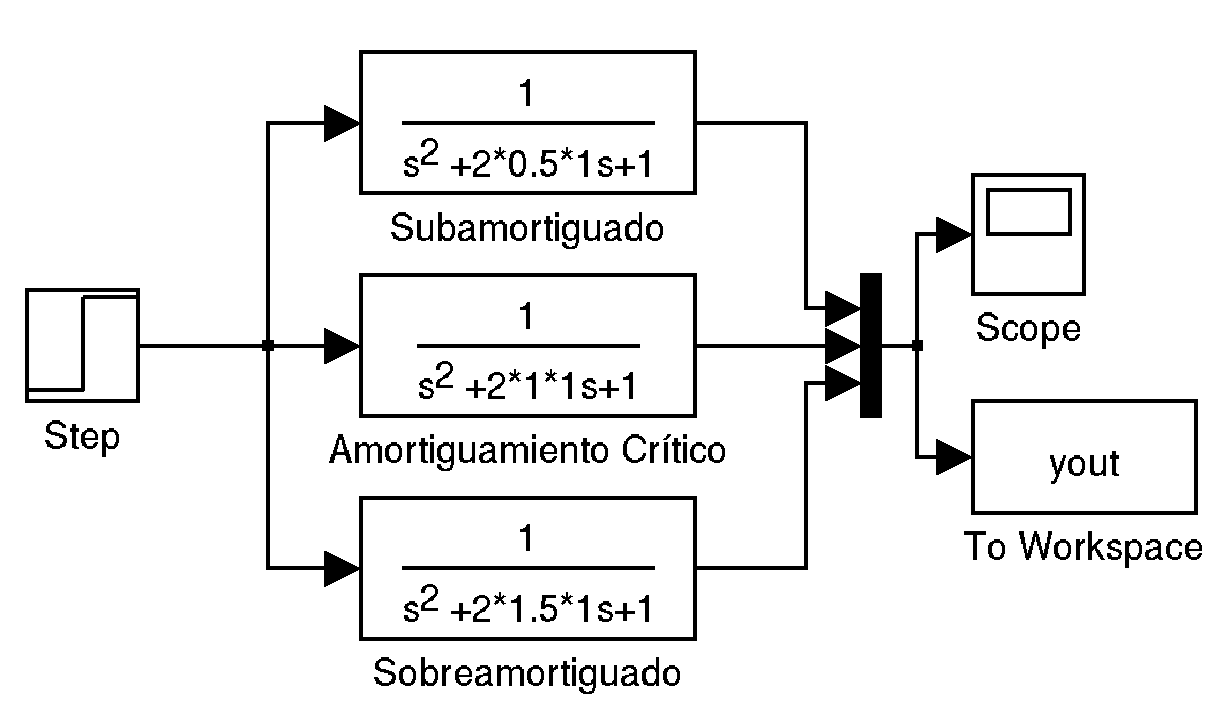
\includegraphics[width=6cm]{imagenes/simulink/simulink_sistemas_segundo_orden.png}
        \caption{Diagrama de bloques.}
    \end{figure}
    \begin{figure}
        \centering
        \scalegraphics{imagenes/respuestas/sistemas_segundo_orden_respuesta_step.png}
        \caption{Respuesta de los sistemas ante una entrada tipo escalón unitario.}
    \end{figure}
    \begin{table}[H]
        \centering
        \begin{tabular}{|c||c|c|c|c|}
            \hline
            & Sobreoscilación & T. Subida & T. Pico & T. Establecimiento 2\%\\
            \hline
            Subamortiguado & 0.1630 & 3.43 & 4.64 & 9.09\\
            \hline
            A. Crítico & -- & -- & -- & 6.85\\
            \hline
            Sobreamortiguado & -- & -- & -- & 11.67\\
            \hline
        \end{tabular}
        \caption{Características de la respuesta temporal de los sistemas.}
    \end{table}
    \section{Funciones de Transferencia con Ceros}
    
    En esta sección se observará el cambio en el comportamiento de la función de transferencia \ref{eq:funcion_transferencia1} que se produce al añadir un cero en el numerador.
    
    \begin{align}
        z_0 = -1~~ &\implies G_1(s) = \frac{s + 1}{s^2 + s + 1}\\
        z_0 = -2~~ &\implies G_2(s) = \frac{0.5\cdot s + 1}{s^2 + s + 1}\\
        z_0 = -5~~ &\implies G_3(s) = \frac{0.2\cdot s + 1}{s^2 + s + 1}\\
        z_0 = -10 &\implies G_4(s) = \frac{0.1\cdot s + 1}{s^2 + s + 1}\\
        z_0 = -20 &\implies G_5(s) = \frac{0.05\cdot s + 1}{s^2 + s + 1}
    \end{align}
    
    %        \begin{figure}[H]
    %            \centering
    %            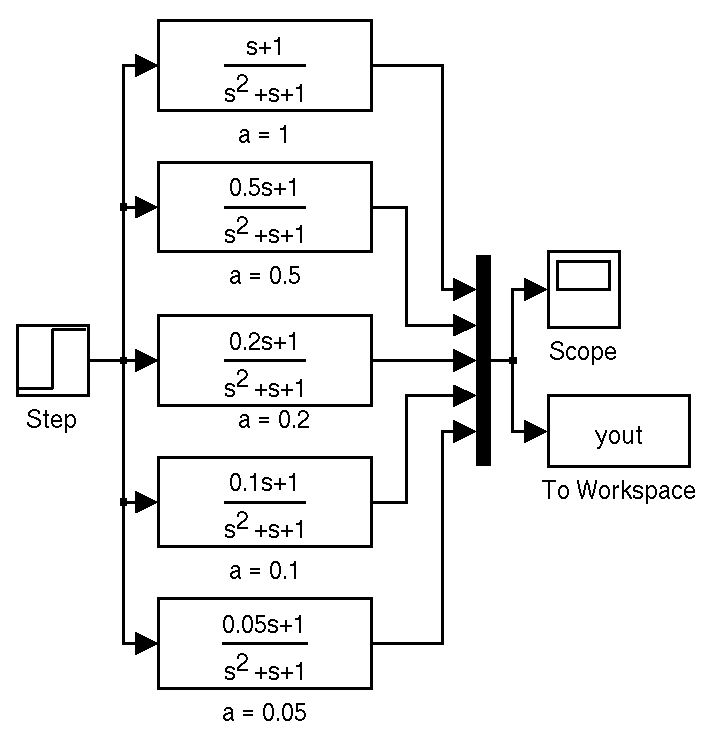
\includegraphics[height = 3cm]{imagenes/simulink/simulink_funciones_de_transferencia_con_ceros.png}
    %            \caption{Diagrama de Simulink de las funciones de transferencia con ceros.}
    %        \end{figure}
    
    
    \begin{figure}[H]
        \centering
        \scalegraphics{imagenes/respuestas/funciones_de_transferencia_con_ceros_respuesta_step.png}
        \caption{Respuestas a un escalón unitario de las funciones de transferencia con ceros.}
    \end{figure}
    A la vista de la representación gráfica de las respuestas de las distintas funciones de transferencia la conclusión es bastante clara, cuanto menor es el cero más despreciable es su aporte. De cualquier forma, sin un problema concreto no se puede determinar la tolerancia permisible. Por lo tanto, basando la decisión en un criterio puramente \emph{ojimétrico}, se puede afirmar que a partir de $Z = -10$ (o incluso $Z = -5$) el cero es despreciable.
    \begin{table}
        \centering
        \begin{tabular}{|c||c|c|c|c|}
            \hline
            & Sobreoscilación & T. Subida & T. Pico & T. Establecimiento 2\% \\
            \hline
            $G_1(s)$ & 0.2984 & 2.22 & 3.43 & 8.52 \\
            \hline
            $G_2(s)$ & 0.1910 & 2.82 & 4.03 & 8.70 \\
            \hline
            $G_3(s)$ & 0.1668 & 3.21 & 4.42 & 8.91 \\
            \hline
            $G_4(s)$ & 0.1639 & 3.32 & 4.53 & 8.99 \\
            \hline
            $G_5(s)$ & 0.1632 & 3.38 & 4.59 & 9.04 \\
            \hline
        \end{tabular}
        \caption{Características de la respuesta temporal de los sistemas.}
    \end{table}
    \newpage
    \chapter{Sistemas Realimentados}
    \section{Sistema Sin controlador}
    \begin{align}
        G(s) = \frac{6}{s^2 + 2s}
    \end{align}
    \begin{figure}[H]
        \centering
        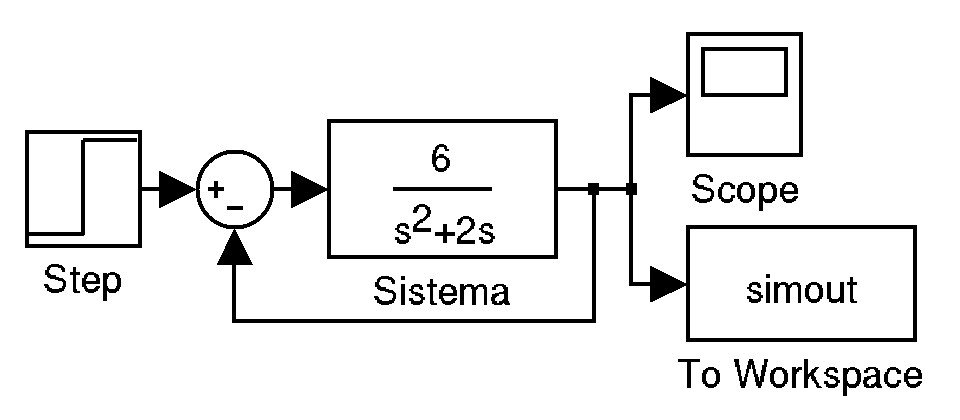
\includegraphics[height = 2.5cm]{imagenes/simulink/simulink_sistema_realimentado_sin_controlador.png}
        \caption{Diagrama de Simulink del sistema.}
    \end{figure}
    \begin{figure}[H]
        \centering
        \scalegraphics{imagenes/respuestas/sin_controlador_respuesta_escalon.png}
        \caption{Respuesta a un escalón unitario del sistema.}
    \end{figure}
    
    \begin{figure}[H]
        \centering
        \scalegraphics{imagenes/respuestas/sin_controlador_respuesta_rampa.png}
        \caption{Respuesta a una rampa unitaria del sistema.}
    \end{figure}
    \begin{table}[H]
        \centering
        \begin{tabular}{|c|c|c|c|c|c|}
            \hline
            Sobreoscilación & T. Subida & T. Pico & T. Establecimiento 2\% & E. Posición & E. Velocidad\\
            \hline
            0.2453 & 1.90 & 2.41 & 4.45 & 0.0193 & 0.3351\\
            \hline
        \end{tabular}
        \caption{Características de la respuesta temporal del sistema.}
        \subsection{Cálculo teórico}
        \begin{align}
            G(s) &= \frac{6}{s^2+2s}\\
            e_p &= \lim\limits_{s \rightarrow 0} s \cdot \frac{1}{s} \cdot \frac{1}{1+\frac{6}{s^2+2s}} = 0\\
            e_v &= \lim\limits_{s \rightarrow 0} s \cdot \frac{1}{s^2} \cdot \frac{1}{1+\frac{6}{s^2+2s}} = \frac{1}{3}
        \end{align}
    \end{table}
    \newpage
    \section{Sistema con controlador PI}
    Sistema controlado por un controlador PI con constantes $K_P=1$ y $K_I=1$
    \begin{align}
        PI(s) &= K_P + \frac{K_I}{s} = \frac{K_Ps + K_I}{s} \implies PI(s) = \frac{s+1}{s}\\
        G(s)  &= \frac{s+1}{s} \cdot \frac{6}{s^2+2s}
    \end{align}
    \begin{figure}[H]
        \centering
        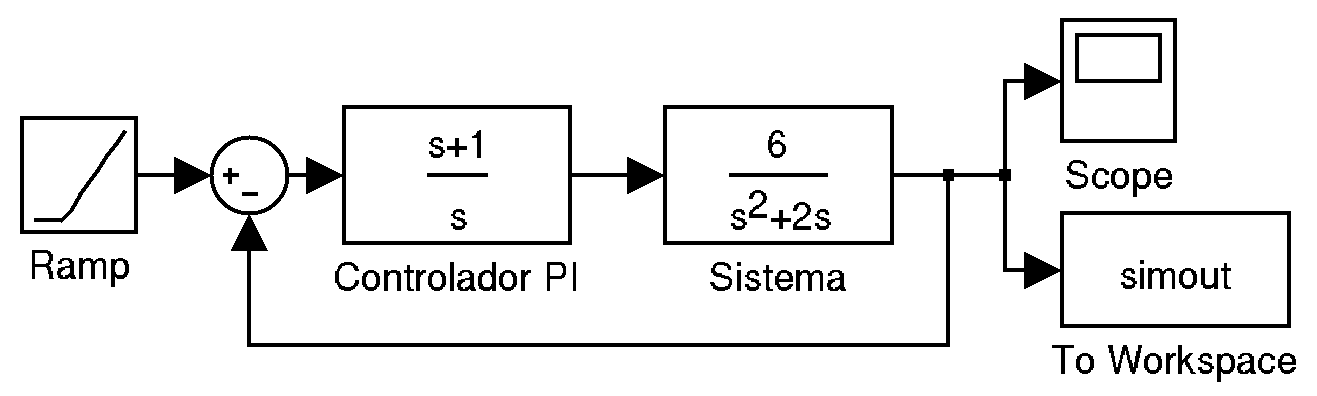
\includegraphics[height = 2.5cm]{imagenes/simulink/simulink_sistema_realimentado_pi.png}
        \caption{Diagrama de Simulink del sistema controlado con PI.}
    \end{figure}
    \begin{figure}[H]
        \centering
        \scalegraphics{imagenes/respuestas/pi_respuesta_escalon.png}
        \caption{Respuesta a un escalón unitario.}
    \end{figure}
    \begin{figure}[H]
        \centering
        \scalegraphics{imagenes/respuestas/pi_respuesta_rampa.png}
        \caption{Respuesta a una rampa unitaria.}
    \end{figure}
    \begin{table}[H]
        \centering
        \begin{tabular}{|c|c|c|c|c|c|}
            \hline
            Sobreoscilación & T. Subida & T. Pico & T. Establecimiento 2\% & E. Posición & E. Velocidad\\
            \hline
            0.6970 & 1.73 & 2.39 & 11.08 & 0.020 & 0.005\\
            \hline
        \end{tabular}
        \caption{Características de la respuesta temporal del sistema simulado.}
    \end{table}
    \subsubsection{Cálculo Teórico}
    %            \begin{align}
    %                E(s) &= X(s) - Y(s)\\
    %                Y(s) &= E(s) \cdot G(s)\\
    %                Y(s) &= [X(s) - Y(s)] \cdot G(S) = X(s)\cdot G(s)-Y(s)\cdot G(s) \rightarrow
    %                Y(s)\cdot(1 + G(s)) = G(s) \cdot X(s)\\
    %                Y(s) &= \frac{G(s)}{1+G(s)} \cdot X(s)\\
    %                E(s) &= X(s) - \frac{G(s)}{1+G(s)} \cdot X(s) = X(s) \cdot \left[1 - \frac{G(s)}{1+G(s)}\right] = \frac{1}{1+G(s)} \cdot X(s)\\
    %                e_p &= \lim\limits_{s \rightarrow 0} s \cdot \frac{1}{1+G(s)} \cdot \frac{1}{s}\\
    %                e_v &= \lim\limits_{s \rightarrow 0} s \cdot \frac{1}{1+G(s)} \cdot \frac{1}{s^2}\\
    %            \end{align}
    %            Para los datos del sistema en cuestión
    \begin{align}
        G(s) &= \frac{s+1}{s} \cdot \frac{6}{s^2+2s} = \frac{6s+6}{s^3+2s^2}\\
        e_p &= \lim\limits_{s \rightarrow 0} s \cdot \frac{1}{s} \cdot \frac{1}{1+\frac{6s+6}{s^3+2s^2}} = 0\\
        e_v &= \lim\limits_{s \rightarrow 0} s \cdot \frac{1}{s^2} \cdot \frac{1}{1+\frac{6s+6}{s^3+2s^2}} = 0
    \end{align}
    \subsection{Reducción de la sobreoscilación}
    Usando métodos de tanteo (iterativos) he llegado a los siguientes valores de las constantes que dejan la sobreoscilación en menos del 10\%
    \begin{align}
        K_P &= 0.41 \\
        K_I &= 0.008
    \end{align}
    \begin{table}[H]
        \centering
        \begin{tabular}{|c|c|c|c|c|c|}
            \hline
            Sobreoscilación & T. Subida & T. Pico & T. Establecimiento 2\% & E. Posición & E. Velocidad\\
            \hline
            0.0918 & 2.83 & 3.63 & 5.35 & 0.0199 & 0.6435\\
            \hline
        \end{tabular}
        \caption{Características de la respuesta temporal del sistema simulado.}
    \end{table}
    \begin{figure}[H]
        \centering
        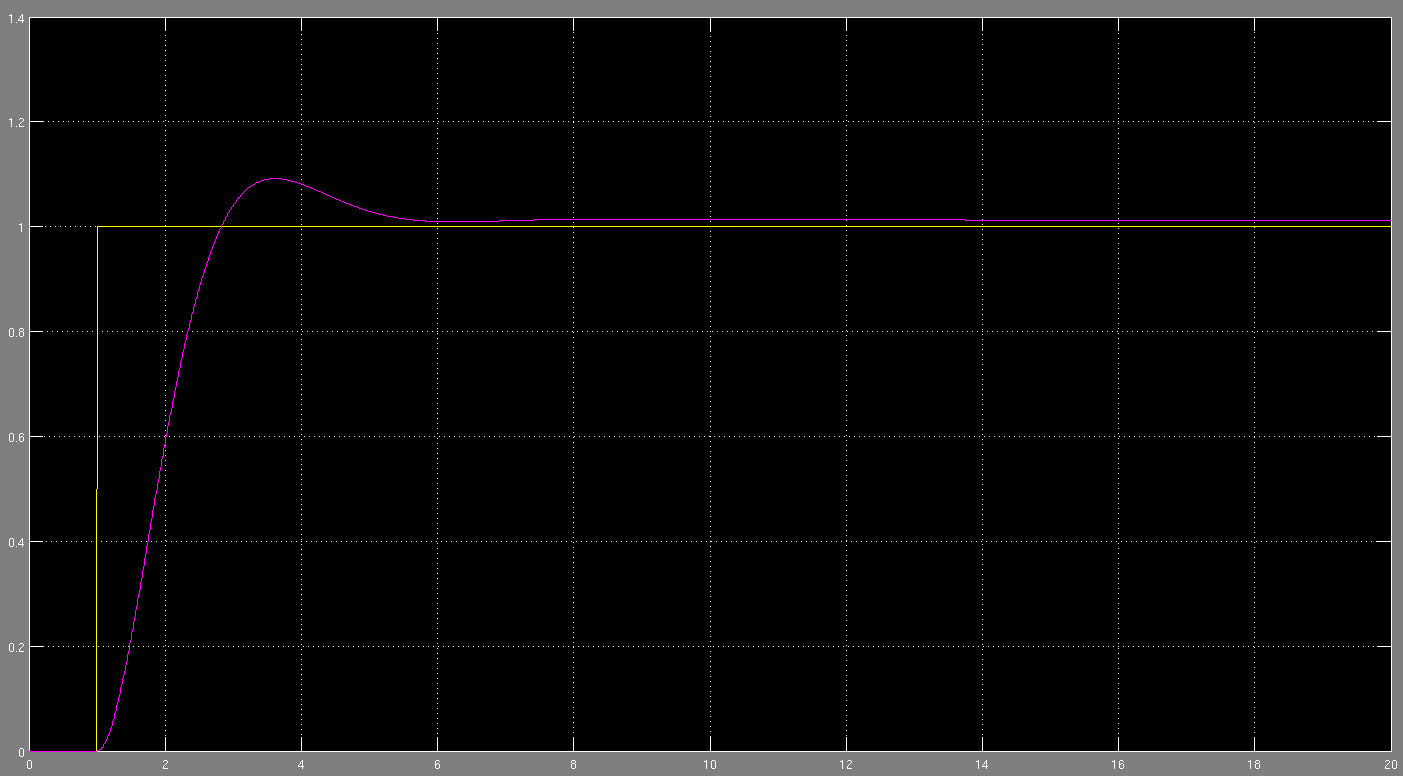
\includegraphics[width = 10cm]{imagenes/respuestas/respuesta_escalon_optimizada.png}
        \caption{Respuesta a una entrada de escalón del sistema optimizado.}
    \end{figure}
    \begin{figure}[H]
        \centering
        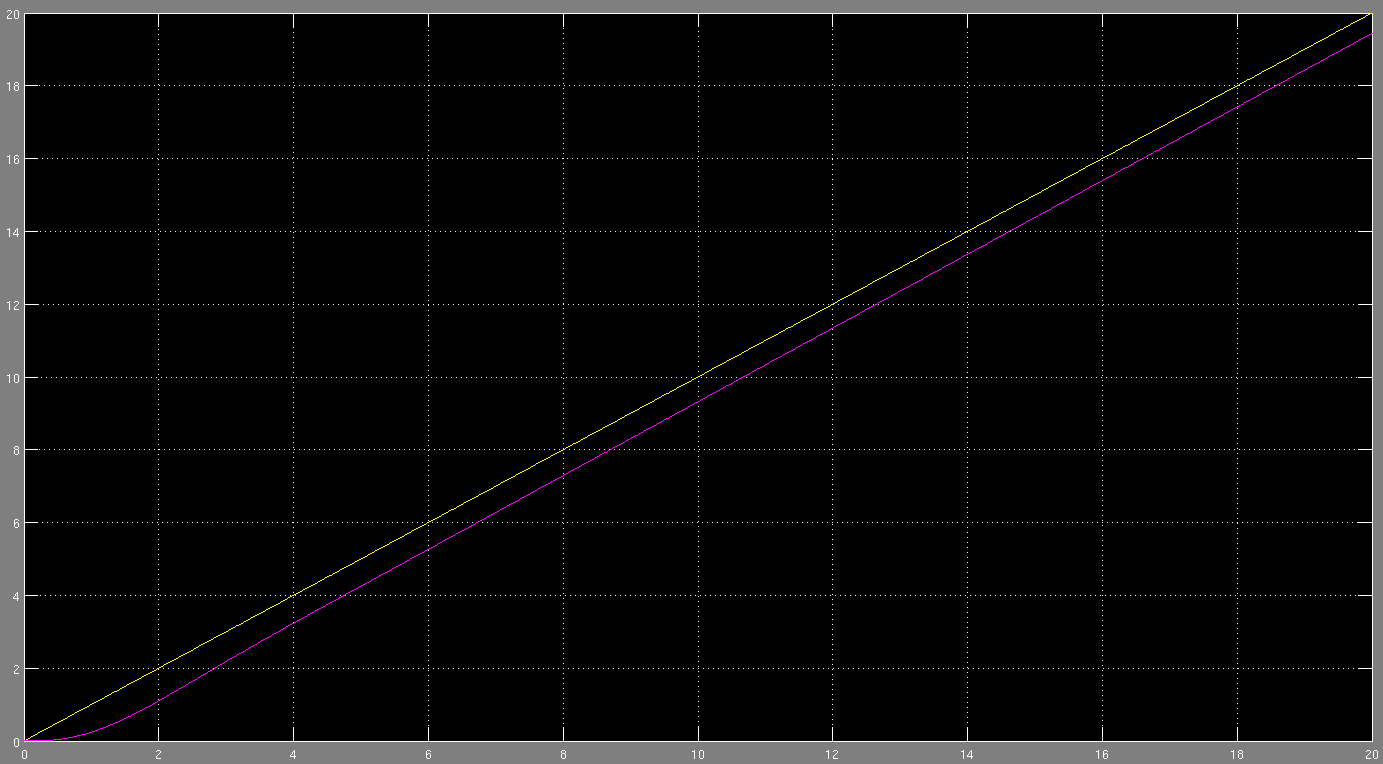
\includegraphics[width = 10cm]{imagenes/respuestas/respuesta_rampa_optimizada.png}
        \caption{Respuesta a una entrada de rampa del sistema optimizado.}
    \end{figure}
    \subsubsection{Cáculo Teórico}
    \begin{align}
        G(s) &= \frac{0.48\cdot s + 0.008}{s} \cdot \frac{6}{s^2+2s} = \frac{2.46 \cdot s + 0.048}{s^3+2s^2}\\
        e_p &= \lim\limits_{s \rightarrow 0} s \cdot \frac{1}{s} \cdot \frac{1}{1+\frac{2.46 \cdot s + 0.048}{s^3+2s^2}} = 0\\
        e_v &= \lim\limits_{s \rightarrow 0} s \cdot \frac{1}{s^2} \cdot \frac{1}{1+\frac{2.46 \cdot s + 0.048}{s^3+2s^2}} = 0
    \end{align}
    \part*{Apéndices}
    \appendix
    \chapter{Código Matlab utilizado}
    \lstinputlisting[language=Matlab]{matlab/sobreoscilacion.m}
    \lstinputlisting[language=Matlab]{matlab/tiempo_pico.m}
    \lstinputlisting[language=Matlab]{matlab/tiempo_subida.m}
    \lstinputlisting[language=Matlab]{matlab/tiempo_establecimiento.m}
    La explicación de la función tiempo\_establecimiento es sencilla, dado el error con respecto a la consigna, el indice a partir del cual la función está dentro del umbral es el siguiente índice al último índice tal que la función está fuera del umbral, es decir, el índice siguiente al índice del último '1' del vector que devuelve (error > umbral).
\end{document}